\documentclass[final]{cmpreport}
\usepackage{algorithm}
\usepackage{algpseudocode}
\usepackage{comment}
\graphicspath{ {./images/} }

\title{GPU Accelerated Method for Constructing and Rendering Trees}
\author{Thomas Mcloughlin}
\date{21/3/2021}
\registration{100203952}
\ccode{CMP - 6013Y}
\supervisor{Dr. Stephen Laycock}

\summary
{
The inclusion of trees in virtual environments when trying to represent nature is 
essential and the branching structure of trees is vital is representing many other 
types of foliage.

This project covers the research of related work involved with algorithmic generation 
of trees and the mathematical basis for the discussed approaches. The underlying 
principles relating to the algorithmic production of fractal patterns helpfully cooincides 
with the requirements for producing believable branching structures. 

The project aim is to convert and extend the Lindenmayer-system based tree construction 
method presented by \citep{prusinkiewicz1996systems} to be used as an independent 
OpenGL module, the intuitive parametric L-system model was chosen because of its 
ability to produce diverse results with varying input. This module allows the addition 
of trees to a real-time environment with minimal user interaction, avoiding the difficulties 
and expenses of manually producing tree models.
}

\acknowledgements
{
I'd like to thank my supervisor, Stephen Laycock for his brilliant help and support 
throughout this project.
Thank you to George Smith and Harry Tucker for their interest in my work and their 
support during the COVID-19 lockdowns. 
}

\begin{document}

\section{Introduction}
This section contains a contextual introduction for the project and a collection of 
related work found during the research phase of development. 

\subsection{Context}
Creating and rendering realistic models of trees manually requires advanced expertise 
with modelling software packages. This limits the ability to produce convincing 3D 
scenes for small developers with restricted resources.

The purpose of including trees in a natural environment is to provide realism. 
Trees are common natural structures present in even simple environments 
throughout the history of computer graphics and have seen many iterations as 
technology has advanced allowing for more detailed and realistic results.

The aim of this project is to provide a method for creating and rendering trees 
to be used in a real-time graphics application. This method should be simple to 
use and implement into an existing OpenGL project.

\subsection{Related Work}
In this subsection various related works will be discussed with respect to how they 
contribute to the main knowledge required for this project, ordered chronologically. 
These areas of main knowledge are the branching structure, branch thickness and leaf 
placement of the constructed trees.

Aristid Lindenmayer proposed an early theory for the development 
of organisms using a cells current state and being combined with input that the cell 
receives from its neighbour \citep{lindenmayer1968mathematical1} \citep{lindenmayer1968mathematical2}. 
Two new cells are produced from this development to replace the existing cell and the 
cycle repeats for the two new cells. 

This process of generating new outputs recursively to produce larger structures became
``Lindenmayer systems'' or the abbreviated ``L-systems'' which became important tools 
in pattern generation for future applications. L-systems became a common approach for the 
generation of branching patterns in flora which is where the aim of this project is 
concerned.

Another early paper that is referenced by many later studies of the subject is by
\cite{honda1971description} where he presented one of the earliest algorithmic 
methods for creating a branching structure. This was done by starting with a parent 
branch which then bifurcates into two child branches and rotating them by given 
angles about the termination point of the parent branch, an example of which 
can be seen in Figure \ref{fig:honda-bifurcation}. By continuing this 
method he treated each child branch as another parent and bifuracted them to 
expand the branching structure which would be continued until a desired result is 
reached.

\begin{figure}[ht]
    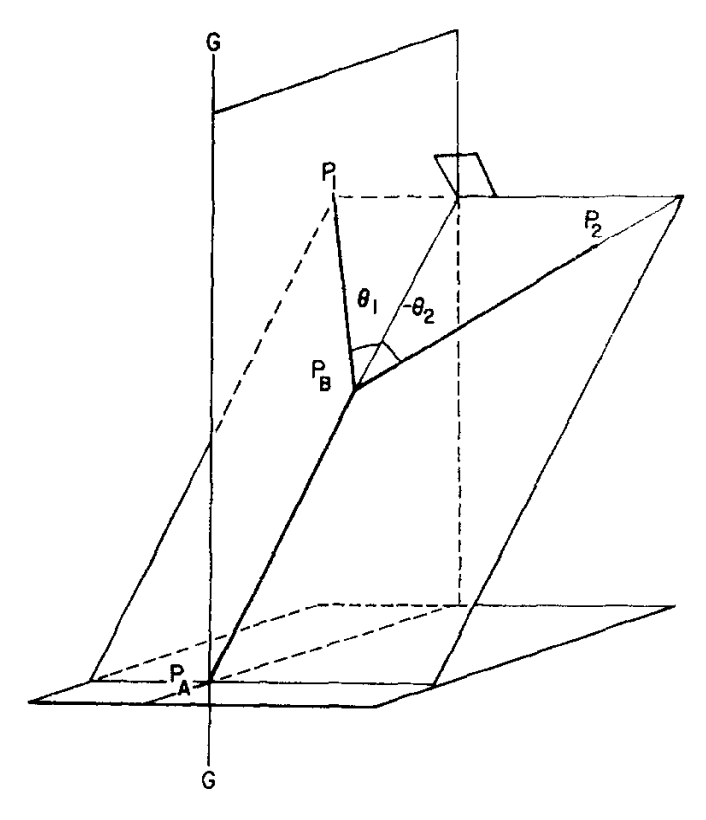
\includegraphics[scale=0.5]{honda-bifurcation.PNG}
    \centering
    \captionsetup{justification=centering}
    \caption{Example diagram of parent branch $P_AP_B$ bifurcating into child branches
    $P_BP_1$ with a rotation of $\theta_1$ and $P_BP_2$ with a rotation of \textminus$\theta_2$.}
    \label{fig:honda-bifurcation}
\end{figure}

This paper does not include any information relating to branch thickness or leaf 
placement as its focus was only on the branching structure. However, this paper 
provides a groundwork for many later studies that will be discussed in this project.

\cite{bloomenthal1985modeling} presents his own tree generation process, specifically 
for a maple tree. He wanted to move beyond simply the branching pattern of a tree which 
most efforts before had focused on \citep{brooks1974geometry,marshall1980procedure,kawaguchi1982morphological,aono1984botanical,smith1984plants}.
For the construction of the branches and trunk he uses splines to create a tree skeleton, 
the use of splines rather than straight lines is chosen to produce a more natural structure. 
He then uses generalised cylinders with varying radii across the splines to create thickness. 
He also describes the use of ramiforms, shown in Figure \ref{fig:bloomenthal-ramiform}, to 
make branch bifurcations realisticly curve rather than have an acute separation.

\begin{figure}[ht]
    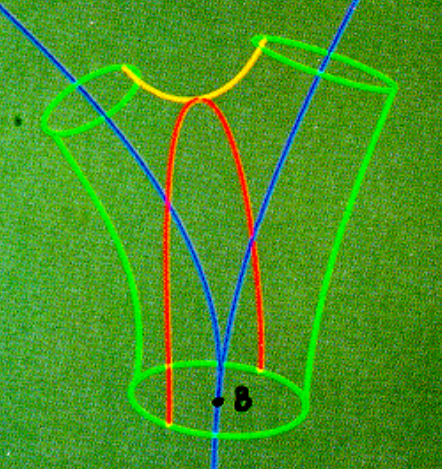
\includegraphics[scale=0.35]{bloomenthal-ramiform.PNG}
    \centering
    \captionsetup{justification=centering}
    \caption{A ramiform used to create a realistic bifurcation.}
    \label{fig:bloomenthal-ramiform}
\end{figure}

The method he describes for leaf placement uses polygonal structures to which he applies 
a leaf texture, these polygons are then brought together in clusters that he calls 
``configurations'' and for each limb that does not exceed a given diameter and that has 
no outgoing limbs, a leaf configuration is chosen at random, scaled randomly and placed 
at the limb tip. The interior lines of each polygon correspond to hinge points of the 
leaves that could be manipulated to show leaf distortion from wind. This method provides 
a more realistic result than the use of simple primitives \citep{kawaguchi1982morphological,lintermann1999interactive,candussi2005rendering}.

\begin{figure}[ht]
    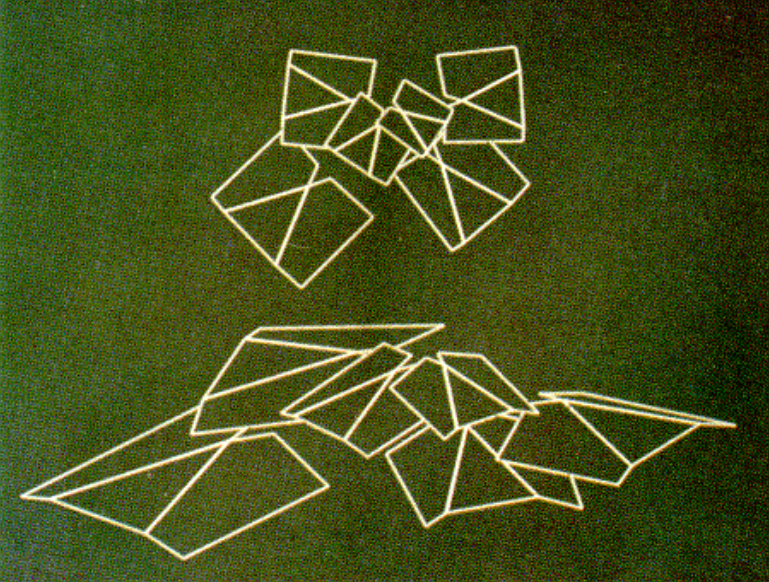
\includegraphics[scale=0.24]{bloomenthal-leaves.PNG} 
    \centering
    \captionsetup{justification=centering}
    \caption{A leaf ``configuration'': plan view (top) and perspective view (bottom).}
    \label{fig:bloomenthal-leaves}
\end{figure}

\cite{prusinkiewicz1996systems} presents a method of tree generation using an advanced 
L-system, developed from the work of \cite{lindenmayer1968mathematical1} and applying 
that system to the bifurcating parent and child branch trios displayed by \cite{honda1971description}.
Their chosen method for representing their models is by using turtle graphics in a 3D 
space and the string generated from the L-system uses symbols that correspond to controlling 
the turtles orientation in space \citep{szilard1979interpretation,prusinkiewicz1986graphical}.

Prusinkiewicz et al. produce a variation on a standard L-system known as a ``deterministic''
L-system or ``D0L-system'' which produces the same result every time. They demonstrate the 
application to turtle graphics with the well-known snowflake curve \citep{mandelbrot1982fractal,koch1906methode} 
shown in Figure \ref{fig:snowflake-lsystem}.

The D0L-system uses an Axiom string and a production rule to recursively develop a longer and 
more complex string. Once a chosen result is reached, the string is traversed and each character 
or group of characters corresponds to the movement of the turtle. Fractals give a convenient 
illustration of the basic workings of an L-system \citep{prusinkiewicz1986graphical,prusinkiewicz2012algorithmic}. 
For example, the D0L-system below represents that of the snowflake fractal where $F(s)$ 
corresponds to a movement forward of distance $s$ and $+(r)$ or $-(r)$ correspond to a rotation 
positively or negatively about the $x$ axis by $r$ degrees.

\textbf{Axiom} $\omega$: $F(1) - (120)F(1) - (120)F(1)$ 

\indent \textbf{Production} $p_1$: $F(s) \rightarrow F(s/3) + (60)F(s/3) - (120)F(s/3) + (60)F(s/3)$

The axiom draws an equilateral triangle with edges of unit length. Production $p_1$ replaces 
each line segment with a polygonal shape where the line segment has been given a convex 
triangular appendage. The Production $p_1$ can be visualised as so:

\begin{figure}[ht]
        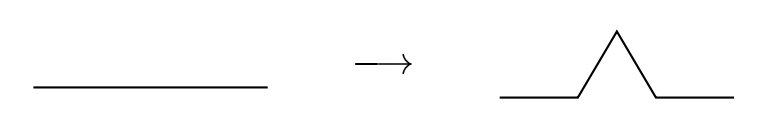
\includegraphics[scale=0.3]{production_p1.PNG}
        \centering
        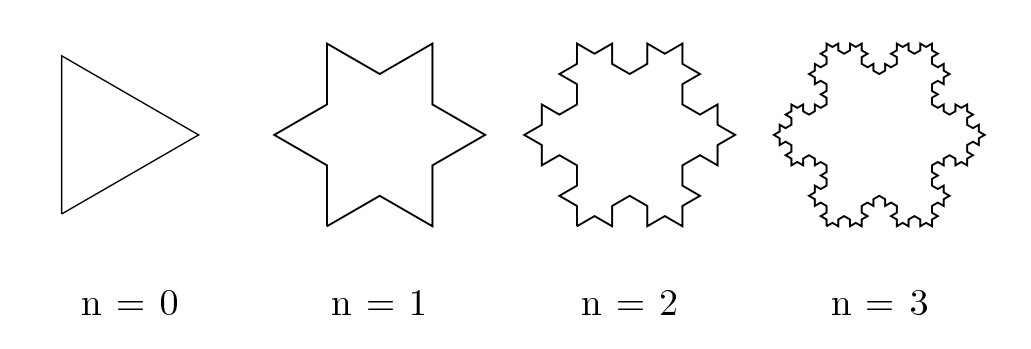
\includegraphics[scale=0.4]{triangle_snowflake_lsystem.PNG}
        \centering
        \caption{The visualised production rule $p_1$, axiom and first 3 recursions 
        defined by the snowflake D0L-system from \citep{prusinkiewicz1996systems} pg.12.}
        \label{fig:snowflake-lsystem}
\end{figure}

Prusinkiewicz et al. go on to present a complex D0L-system to be used for constructing 
tree structures by creating a Parametric L-system allowing for input to alter the axiom 
string producing different results along with using a conditional requirement to 
decide automatically when to stop recursing. 

This L-system is defined below, in this 
context $A(s, w)$ refers to a line segment or ``apex'' of length $s$ and width $w$. 
Production $p_1$ begins with the conditional statement to only continue if the length $s$ 
of the current apex is greater than or equal to $min$ which is a chosen minimum length. If 
the condition is met then $!(w)F(s)$ draws a line of length $s$ and width $w$. 

Lines $a_1$ and $a_2$ refer to the bifurcated child apices of the parent apex which are 
given a rotation of $\alpha_1$ and $\alpha_2$ radians about the $x$ axis and a rotation of 
$\phi_1$ and $\phi_2$ radians about the $y$ axis. The length of the child apices is calculated 
by multiplying the parent apex length $s$ by the corresponding length degradation parameters 
$r_1$ and $r_2$ respectively. A degradation in width is calculated using $q$ and $e$.

$\omega$: $A(100, w_0)$ 

\indent $p_1$: $A(s, w) : s >= min \rightarrow !(w)F(s)$

\indent $a_1$ $[+(\alpha_1)/(\phi_1)A(s * r_1, w * q ^ e)]$

\indent $a_2$ $[+(\alpha_2)/(\phi_2)A(s * r_2, w * (1 - q) ^ e)]$

This L-system is used to produce various complex tree patterns, shown in section 
\ref{app:parameterised-lsystem-trees} of the Appendix, ranging from mathematical fractal 
patterns to some realistic looking structures.

Prusinkiewicz et al. do not directly propose a method of leaf placement as this 
paper focuses on tree structure and the manipulation of L-systems, they do however provide 
an example where terminating apices of an L-system could be replaced with a leaf shape to 
give a rudimentary leaf placement approach.

\cite{weber1995rendering} produced a model for creating and rendering trees that emphasises 
overall geometric structure of the tree rather than strictly following botanical principles 
which they credit similarity to the aims of \cite{reeves1985approximate}. 
They admit that their model resembles that proposed by \cite{oppenheimer1986real} which used 
fractals with parameters such as ``branching angle'' and ``helical twist'' to produce trees. 
However, Weber et al. propose that the use of fractal theory self similarity by Oppenheimer 
is not necessesary and restricts results to only a small number of basic trees.

Weber et al. used cylinders and cones as branch segments, 
each child branches base circle coinciding with the top circle of the parent branch. 
Transformation of the child branches being controlled through the intentionally intuitively named 
parameters that can be edited by the user to produce a desired result.

Figure \ref{fig:weber-splits} shows some of the many parameters that can be used to affect 
tree generation, \emph{0SegSplits} defines the number of splits at each branch termination, 
\emph{0SplitAngle} controls the angle at each split, \emph{0CurveRes} refers to the taper 
given to each branch to slowly reduce thickness of each branch, and \emph{1Rotate} defines 
the $y$ axis rotation of the branch. The number in front of each parameter refers to a branch, 
0 being the root branch, the values of parent branch parameters are passed on to the child 
branches. 

\begin{figure}[ht]
    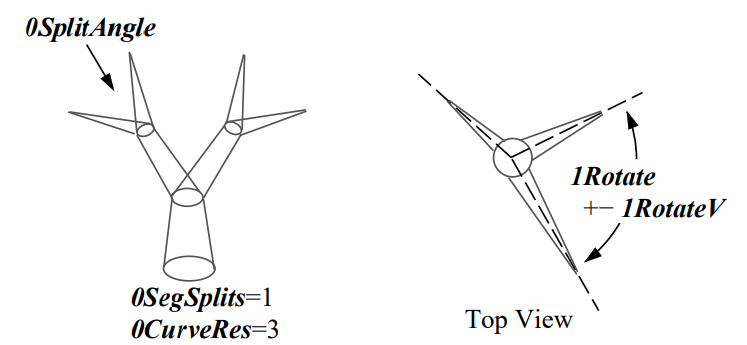
\includegraphics[scale=0.5]{weber-splits.PNG} 
    \centering
    \captionsetup{justification=centering}
    \caption{Example of tree parameters.}
    \label{fig:weber-splits}
\end{figure}

Leaf placement is handled using a ``Level'' system that refers to the number of recursions from 
the root branch. If a parameter \emph{Leaves} is non-zero then the final level of recursion is 
used to place leaves on the final set of child branches, using a set of leaf specific parameters 
to control the rotation of each leaf. The shape of the leaves is controlled using the parameter 
\emph{LeafShape} allowing for different tree species to be represented by adding different leaf 
shapes.
\cite{weber1995rendering} served as a groundwork for many future approaches and advances in tree 
rendering \citep{remolar2004rendering,wesslen2005real}. Weber himself went on to produce a 
simulation focused method of tree generation including some extra features such as branches 
avoiding obstacles \citep{weber2008simulation}.

Another branch structure method, that differs uniquely from methods mentioned above, is that of 
space colonisation \citep{runions2007colonization}. The steps of this method can be seen in Figure \ref{fig:space-colonisation} 
and works by producing a three-dimensional envelope to be used for the tree crown containing a set 
of ``attraction points'' which are used as targets for branch growth. The tree skeleton interatively 
expands by producing new branches in the direction of the attraction points. Once an attraction point 
is reached by a branch, the point is removed and the branch terminates. This process is continued 
until all attraction points are reached, when no new branches are within attraction radius of 
remaining points or when a user inputted number of iterations has been reached. 

\begin{figure}[ht]
    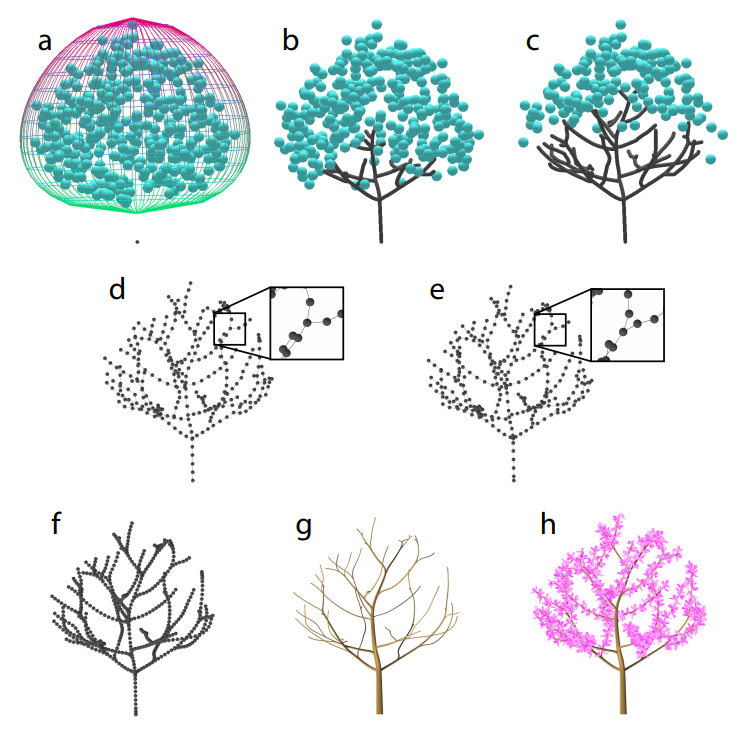
\includegraphics[scale=0.5]{space-colonisation.PNG} 
    \centering
    \captionsetup{justification=centering}
    \caption{Space colonisation steps.}
    \label{fig:space-colonisation}
\end{figure}

Once a tree skeleton has been finalised they determine the width of the limbs using the pipe 
model \citep{shinozaki1964quantitative} and the tree geometry is modeled using generalised 
cylinders \citep{bloomenthal1985modeling}.

A leaf placement method is not provided as part of this paper due to it focusing solely on 
branch construction. However, they do suggest that the placement density of leaves or flowers 
could be controlled using absolute distance from the root position to give a realistic dispersion 
of leaves throughout the tree crown.

\section{Design and Development}
After going through the relevant related work, the chosen method for constructing the trees was 
using an L-system. This was chosen because a complex parameterised L-system could be designed to 
produce various different types of trees while using the same logic pipeline. Therefore, the 
module could be relatively simple and contained, and still be quite flexible with its results.

Using an L-system meant that a basic branch object was needed to construct each section of the 
tree. The first approach investigated was the use of quadric cylinders, that could be 
used to give branches thickness. Quadric cylinders could also be defined with a taper allowing 
for a smooth reduction in thickness towards external branches. Figure \ref{fig:quadric-cylinders} shows 
an early test bifurcation using quadric cylinders.

\begin{figure}[ht]
    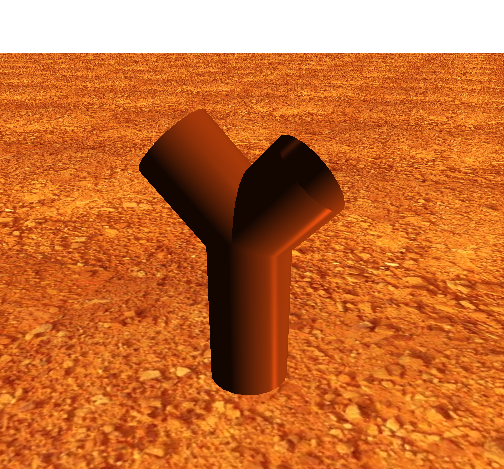
\includegraphics[scale=0.5]{quadric-cylinders.png} 
    \centering
    \captionsetup{justification=centering}
    \caption{3 quadric cylinders positioned as a bifurcation.}
    \label{fig:quadric-cylinders}
\end{figure}

When positioned correctly, the join between 
overlapping cylinders was acceptably smooth producing a believable bifurcation. However, this 
example was made by hardcoding transformation for each quadric that was applied separately with 
no direct relationship between the parent and child branches. The quadric class was also closed 
off from being modified, meaning that the construction method would be restricted to however the 
quadrics can be manipulated and I would not be able to make any tweaks to how the quadrics are 
constructed to assist with the L-system generation. Another foreseen difficulty was the issue of
texturing, which would me more complex when using quadrics.
Because of this the decision was made to instead create a cylinder class specifically for this 
purpose, therefore allowing better control of generating the models and allowing for tweaks to 
made when integrating them with the L-system. 

The cylinder class was intially designed to produce a line rather than an entire cylinder so that 
testing could be carried out more quickly and tree skeletons would be easier to analyse for 
mistakes in the L-system. Unfortunately the cylinder class did not advance further than using 
lines for the construction but this will be explained in the Evaluation. 

These cylinder objects are constructed using vertex array objects and vertex buffer objects with 
the aim of being able to store the geometry data of a constructed tree as a vector of these 
objects and then simply interate through and load each cylinder object. The cylinder object is 
constructed using a glm::vec3 for the base and top centre point of the cylinder, and has a top 
and bottom radius that would be used to control tapering. 

To test the use of this cylinder class and develop understanding of L-system production some 
basic L-systems were produced. These included a basic binary tree, and a barnsley fern L-system.
The L-system for a binary tree is displayed below.

\begin{figure}[ht]
    Binary Tree L-system:

    $\omega$: $a$ 

    $p_1$: $a \rightarrow b[a]a$

    $p_2$: $b \rightarrow bb$
    \label{fig:b-tree-string-system}
\end{figure}

These production rules are applied for a set number of recursions to control the size of the 
resulting tree. The first 3 recursions of this system, with an axiom of $a$, are:

1: b[a]a

2: bb[b[a]a]b[a]a

3: bbbb[bb[b[a]a]b[a]a]bb[b[a]a]b[a]a

Each character refers to a certain action when constructing the tree. In this case a means draw 
a branch segment terminating with two small lines to represent a leaf, b means draw a branch 
segment, $[$ means push position and angle and rotate 45 degrees left about $x$ and $]$ means 
pop position and angle and rotate 45 degrees right about $x$. Six recursions using this system 
produces the binary tree shown in Figure \ref{fig:b-tree-fern-string}, and you can see the 
steps used to construct the tree using this method in section \ref{app:b-tree-lsystem-algo}.

A somewhat more advanced L-system, used to test whether the line segments can produce a more natural 
shape, is an L-system designed to create an adapted version of the Barnsley fern fractal. The 
production rules for this L-system are shown below.

\begin{figure}[ht]
    Barnsley Fern L-system:

    $\omega$: $a$ 

    $p_1$: $a \rightarrow b+[[a]-a]-b[-ba]+a$

    $p_2$: $b \rightarrow bb$
    \label{fig:b-fern-string-system}
\end{figure}

This L-system produces a natural looking branched fern pattern, shown in Figure \ref{fig:b-tree-fern-string}. 
This proves that this method of line segments can be used for this projects aim.

\begin{figure}[ht]
    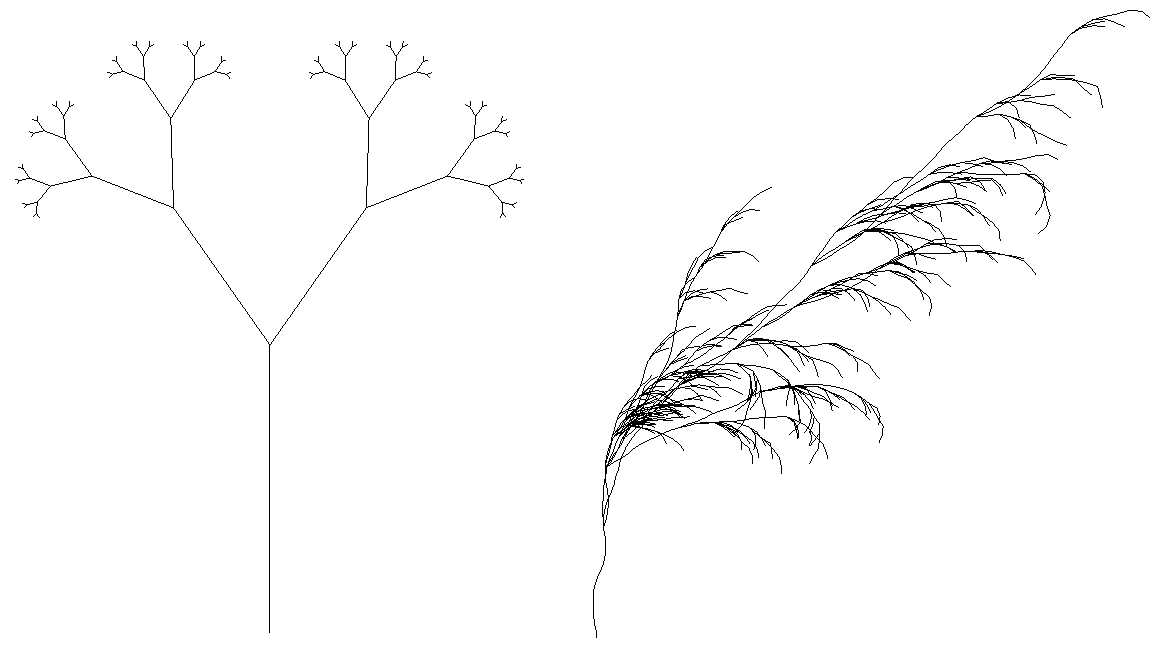
\includegraphics[scale=0.4]{b-tree-fern-string.png} 
    \centering
    \captionsetup{justification=centering}
    \caption{Binary Tree L-system result after six recursions (left) and Barnsley Fern L-system
             after five recursions (right).}
    \label{fig:b-tree-fern-string}
\end{figure}

Having confirmed the effectiveness of the cylinder class to produce lines correctly, the next 
step was to produce a more advanced L-system to create more details structures and make the 
transition to 3D. 

The decision was made to adapt the parametric L-system described by \cite{prusinkiewicz1996systems}, 
discussed in the related work section, into OpenGL using the cylinder class to generate lines. 
This required developed understanding of L-systems and adaptation from the proposed turtle graphics
approach, over to using OpenGL vertices.

This parametric L-system was described in the related work section but will be re-iterated with 
respect to it's adaptation in OpenGL.

$\omega$: $A(100, w_0)$ 

\indent $p_1$: $A(s, w) : s >= min \rightarrow !(w)F(s)$

\indent $a_1$ $[+(\alpha_1)/(\phi_1)A(s * r_1, w * q ^ e)]$

\indent $a_2$ $[+(\alpha_2)/(\phi_2)A(s * r_2, w * (1 - q) ^ e)]$

The initial approach taken was to try and implement the classical L-system result of string 
generation and then producing results by iterating through the resulting string, such as the 
binary tree and barnsley fern described above. However, after an attempted implementation of 
this approach, the decision was made to switch to an object oriented construction.

The L-system production rules takes an ``Apex'' defined as $A(s, w)$ and produces the two child 
apices $a_1$ and $a_2$ which are then also passed through the production rules to produce their 
own child apices. This proved clumsy when trying to use strings and therefore an Apex class was 
created to represent the relevant data of each Apex that could then be used to construct the 
branches. 

The data defined in the Apex class includes: 
\begin{itemize}
    \item The \emph{length} and \emph{width} of the branch.
    \item The \emph{rotateAlpha} and \emph{rotatePhi} which refer to the rotation about the $x$ and $y$ axis 
          respectively.
    \item Pointers to the parent Apex and child apices.
    \item The \emph{localRoot} of the Apex which is a glm::vec3 used to represent the 3D coordinates 
          of the base of the branch.
    \item The integer \emph{level} that stores the number of recursions away and Apex is from the root Apex.
    \item A boolean \emph{isRoot} to check whether an Apex is the root Apex or not.
    \item A rotation matrix used to rotate apices using \emph{rotateAlpha} and \emph{rotatePhi} with 
          respect to the cumulative rotations of the parent Apex.
\end{itemize}

These apices are used to create the line segments required to generate the tree structure. The 
Line segments are stored in a vector and then, when loading the scene, iterated through to render the tree.

The parameters required for this L-system are passed into a function and then used to construct 
the Apex object necessary for the tree. These variables are:

\begin{itemize}
    \item \emph{rootPos}, a glm::vec3 representing the 3D coordinates where you want the tree to be rendered.
    \item \emph{startBranchLength}, the starting length of branches.
    \item \emph{minBranchLength}, the minimum branch length used to check the conditional statement in the 
          L-system, if the current branch length is lower than the minimum then the system stops recursing.
    \item \emph{startBranchWidth}, the starting branch width.
    \item \emph{angleAlpha1} and \emph{angleAlpha2} control rotations about the $x$-axis.
    \item \emph{anglePhi1} and \emph{anglePhi2} control rotations about the $y$-axis.
    \item \emph{lengthDegrade1} and \emph{lengthDegrade2} control the rate at which the length of branches 
          degrades from parent to child.
    \item \emph{count}, used to control the number of recursions directly if the minimum length approach 
          is not suitable.
\end{itemize}

Alterations of these variables can be used to produce vastly different outcomes as shown by the 
results of \cite{prusinkiewicz1996systems}, which are included in section \ref{app:parameterised-lsystem-trees}.

To construct the apices vector, these variables are passed through to a recursive function that 
creates each Apex object, sets parent and child relationships, and handles length degredation.
This function used to construct the apices vector is shown in section \ref{app:construct-tree}. 
The initial implementation for constructing the apices vector used a simple loop, this made 
setting parent-child relationships unecessarilly obtuse however. Therefore the recursive method 
was developed to streamline the construction process and also improve readability of the code.

Having constructed the apices vector the last step was to iterate through each Apex and use their 
data to render a line. This is where most issues arose in development as multiple iterations were 
used for applying rotations before a working solution was found.

\cite{prusinkiewicz1996systems} used a proprietary coordinate system to describe their transformations 
when using turtle graphics and those axes are shown in Figure \ref{fig:uhl-coords}. For reference 
the axes $u, h, l$ correspond to $x, y, z$ respectively. 

The rotations discussed below only display rotations about the $x$ and $y$ axes because these 
are the only two rotations involved in this L-system.

\begin{figure}[ht]
    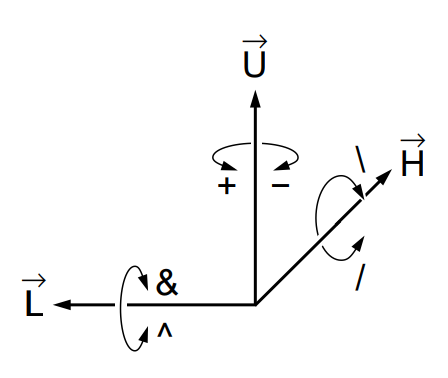
\includegraphics[scale=0.4]{uhl-coords.PNG} 
    \centering
    \captionsetup{justification=centering}
    \caption{Axes used to control the turtle in three dimensions.}
    \label{fig:uhl-coords}
\end{figure}

\pagebreak
Initially, rotations were applied by calculating the rotation of each element of the coordinate,

For the $x$-axis:

$x = x$

$y = y\cos(rotationAlpha) - z\sin(rotationAlpha)$

$z = y\sin(rotationAlpha) + z\cos(rotationAlpha)$

For the $y$-axis:

$x = x\cos(rotationPhi) + z\sin(rotationPhi)$

$y = y$

$z = z\cos(rotationPhi) - x\sin(rotationPhi)$

These were then simplified to complete all rotations with just one calculation for each element 
rather than having to run separate calculations for \emph{rotationAlpha} and \emph{rotationPhi}.

$x = length\cos(rotationPhi)\sin(rotationAlpha)$

$y = length\sin(rotationPhi)\sin(rotationAlpha)$

$z = length\cos(rotationAlpha)$

The final method that proved successful was the use of rotation matrices as part of the Apex 
objects with the glm::rotate function. When the parent of a child Apex is set in the apices vector 
construction process, the rotation matrix of the child is calculated using the rotation matrix 
of the parent so that the angle of the parent branch is taken into account. 

The code below is a simplification of glm::rotate and assumes local variables of an 
Apex object, rotation values are converted to radians for use with glm::rotate and the last 
parameter refers to the axis of rotation shown $x, y$ however, in code this would be 
a glm::vec3 with a 1 in the parameter corresponding to the chosen axis.

Alpha rotation:

$rotationMatrix = rotate(parentRotationMatrix, rotationAlpha, x)$

Phi rotation:

$rotationMatrix = rotate(rotationMatrixAlpha, rotationPhi, y)$

The rotation Matrix of an Apex object can then be used to rotate a point for creating a line 
segment along with the other Apex attributes. The algorithm below displays how the apices 
vector is used to create lines ready to be rendered into a scene.

\begin{figure}[ht]
    \begin{algorithm}[H]
    \caption{constructLines(\emph{apices}) {\textbf{return}} \emph{lines}}
        \begin{algorithmic}[1]
        \Require $apices$, vector of Apex objects
        \Ensure \emph{lines}, vector of line objects
        \ForAll{$Apex$ in $apices$}
            \State \emph{top} $\leftarrow ApexRotationMatrix * (0, ApexLength, 0, 1)$ 
            \State \emph{top} $\leftarrow (topX + ApexX, topY + ApexY, topZ + ApexZ)$ 
            \State \emph{newLine} $\leftarrow generateLine(ApexLocalRoot, top)$ 
            \State Push \emph{newLine} onto \emph{lines}
            \If{\emph{Apex} has first child}
                \State Set \emph{Apex} first child \emph{localRoot} to \emph{top}
            \EndIf
            \If{\emph{Apex} has second child}
                \State Set \emph{Apex} second child \emph{localRoot} to \emph{top}
            \EndIf
        \EndFor
        \State \Return \emph{lines}
        \end{algorithmic}
    \end{algorithm}
    \caption{Construction of line segments ready for rendering.}
    \label{fig:construct-lines}
\end{figure}

The code pipeline has also been designed so that if new L-systems were needed then they could 
be implemented as part of a new \emph{L-system} object. This was done to allow for future 
adopters of the module to expand the source code to meet their requirements.

\section{Analysis of Results}
I this section, three different trees will be analysed for their performance and then analysed 
when all three trees are loaded at once. These trees are results from the method desribed in 
the previous section, and are examples taken from \cite{prusinkiewicz1996systems} to allow 
benchmarking in the evaluation section.

\subsection{Short Tree}
The first tree, shown in Figure \ref{fig:tree-g}, has a short, wide crown with an even spread of branches.
Alterations to this structure would produce results close to that of an ash tree. 

\begin{figure}[ht]
    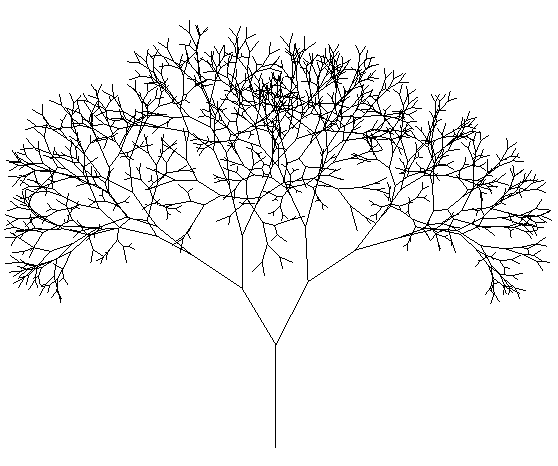
\includegraphics[scale=0.7]{tree-g.PNG} 
    \centering
    \captionsetup{justification=centering}
    \caption{Short Tree.}
    \label{fig:tree-g}
\end{figure}

The performance of this tree and others was measured using the built in diagnostics tools in 
the visual studio editor. An empty scene has been measured at a memory usage of 43MB so the 
results included are the total usage with the base 43MB subtracted. 

The short tree has a consistent memory usage of 65.4MB, and subtracting the base usage of 43MB gives 
us a usage of 22.4MB. CPU utilization fluctuates between 6\% and 9\%, and when rotated the tree 
does not cause a reduction in frames per second.

\subsection{Medium Tree}
The next tree, shown in Figure \ref{fig:tree-h}, is a medium sized tree with some main spreading 
branches but has a lower length degredation than the short tree causing it to grow taller. This 
structure could be used to represent a maple tree.

\begin{figure}[ht]
    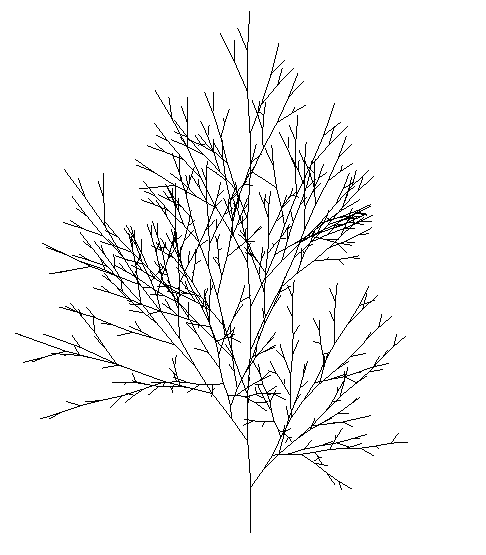
\includegraphics[scale=0.7]{tree-h.PNG} 
    \centering
    \captionsetup{justification=centering}
    \caption{Medium Tree.}
    \label{fig:tree-h}
\end{figure}

The medium tree has a memory usage of 56.9MB, real usage 13.9MB. Fluctuates between 6\% and 
9\% CPU utilization, and when rotated does not cause a reduction in frames per second.

This tree has a higher minimum branch length than the short tree, meaning that less branch 
segments are generated, which is why the memory usage is lower.

\pagebreak
\subsection{Tall Tree}
The third tree, shown in Figure \ref{fig:tree-i}, is a tall tree with less widely spreading 
branches that have shorter child segments making the tree stand tall and compact with minimal 
overhang from the trunk. The structure below would be well suited for creating a birch tree.

\begin{figure}[ht]
    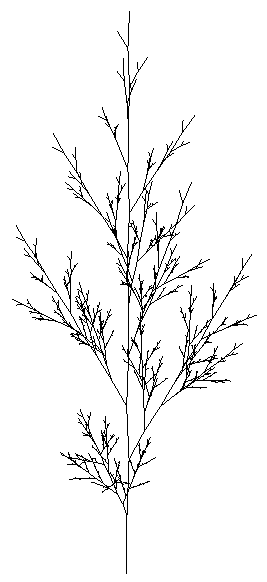
\includegraphics[scale=0.7]{tree-i.PNG} 
    \centering
    \captionsetup{justification=centering}
    \caption{Tall Tree.}
    \label{fig:tree-i}
\end{figure}

The tall tree has a memory usage of 63.6MB, real usage 20.6MB. Fluctuates between 6\% and 9\% 
CPU utilization, and when rotated does not cause a reduction in frames per second.

This tree has a minimum branch length greater than the short tree but less than the medium tree,
hence the memory usage being between that of the previous examples.

\pagebreak
\subsection{Multiple Trees}
The final test was to take multiple tree models and load them into the same scene. This is 
important to test as an evironment containing trees is likely to contain more than one, such as 
a forest. Figure \ref{fig:trees-ghi} shows a scene with all three of the previously analysed 
trees loaded in at once. 

\begin{figure}[ht]
    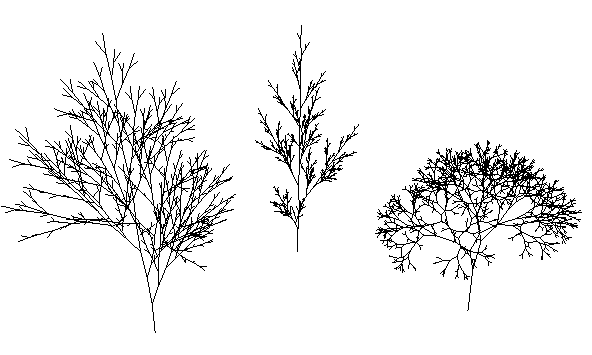
\includegraphics[scale=0.7]{trees-ghi.PNG} 
    \centering
    \captionsetup{justification=centering}
    \caption{Medium (left), Tall (centre) and Short (right) trees.}
    \label{fig:trees-ghi}
\end{figure}

This scene requires more resources to load than a singular tree with a memory usage of 89MB. 
Worth noting is that with the 89MB measurement, subtracting the base 43MB gives us a usage of 
46MB which does not cooincide with an addition of each trees separate memory usage.
This is likely due to every tree being stored in a single vector.

This scene fluctuates CPU utilization between 6\% and 9\% for the first 5 seconds 
approximately before steadying at 6\%. For the first few seconds this scene has some frame 
slowdowns and loads slower than the previous examples.

\section{Discussion and Evaluation}


\section{Conclusion}


%Bibliography
\pagebreak
\bibliography{bibfile}

%Appendix
\appendix{}
\begin{figure}[ht]
    \section{Parameterised L-system Trees}
    \label{app:parameterised-lsystem-trees}
    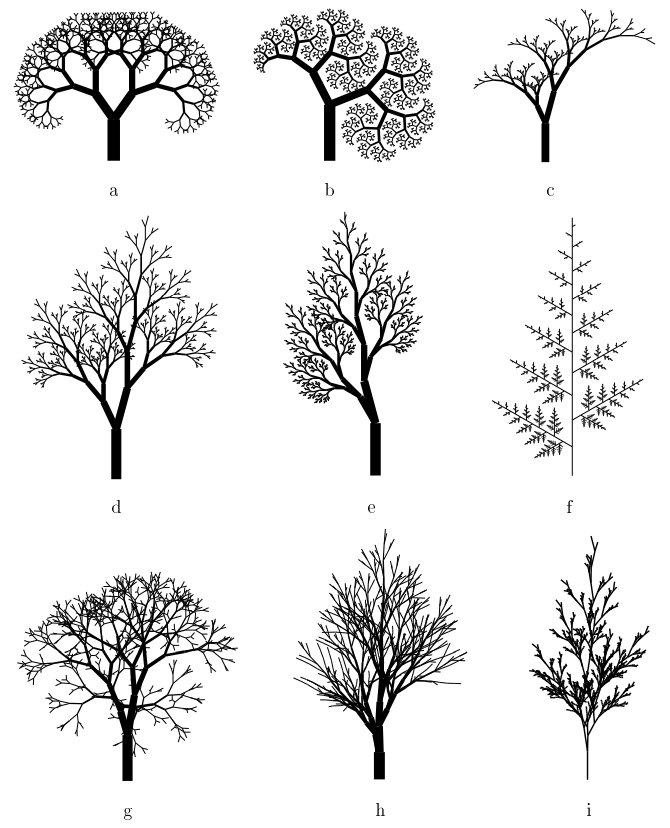
\includegraphics[scale=0.7]{tree-lsystem-results.PNG} 
    \centering
    \captionsetup{justification=centering}
    \caption{Tree structures produced using the proposed L-system described by \cite{prusinkiewicz1996systems}}
    \label{fig:tree-lsystem-results}
\end{figure}

\begin{figure}[ht]
    \section{Binary Tree L-system Algorithm}
    \label{app:b-tree-lsystem-algo}
    \begin{algorithm}[H]
    \caption{generateBinaryTree(\emph{axiom, numRecursions}) {\textbf{return}} \emph{branchList}}
        \begin{algorithmic}[1]
        \Require $axiom$, the initial string for the L-system
        \Require $numRecursions$, number of times to run production rules
        \Ensure \emph{branchList}, list of branch objects that can be rendered
        \State $systemString \leftarrow getLsystemString(axiom, numRecursions)$
        \State $currentPosition \leftarrow$ bottom of tree
        \State $rotationX \leftarrow 0$
        \State $positionList$, $angleList$ 
        \ForAll{$character$ in $systemString$}
            \If{$character$ = $a$}
                \State $newBranch \leftarrow$ short terminating branch
                \State rotate $newBranch$ by $rotationX$ about $x$-axis
                \State translate bottom of $newBranch$ to $currentPos$
                \State push $newBranch$ onto $branchList$
            \ElsIf{$character$ = $b$}
                \State $newBranch \leftarrow$ long branch
                \State rotate $newBranch$ by $rotationX$ about $x$-axis
                \State translate bottom of $newBranch$ to $currentPos$
                \State push $newBranch$ onto $branchList$
                \State $currentPos \leftarrow$ top of $newBranch$
            \ElsIf{$character$ = $[$}
                \State push $currentPos$ onto $positionList$
                \State push $rotationX$ onto $angleList$
                \State $rotationX \leftarrow rotationX + 45$
            \ElsIf{$character$ = $]$}
                \State pop $positionList$ to $currentPos$
                \State pop $angleList$ to $rotationX$
                \State $rotationX \leftarrow rotationX - 45$
            \EndIf
        \EndFor
        \State \Return $branchList$
        \end{algorithmic}
    \end{algorithm}
    \caption{Construction method with Binary Tree L-system}
\end{figure}

\begin{figure}[ht]
    \section{Construct Apices Vector}
    \label{app:construct-tree}
    \begin{algorithm}[H]
    \caption{constructTree(\emph{root, apices, a1, a2, p1, p2, l1, l2, r1, r2, min, w1, w2, count}) {\textbf{return}} \emph{branchList}}
        \begin{algorithmic}[1]
        \Require $root$, parent Apex of this recursion
        \Require $apices$, current vector of all generated apices
        \Require Generation variables, explained in the caption below
        \Ensure \emph{apices}, vector of Apex objects
        \State Create new Apex object \emph{apex1} with variables \emph{a1, p1, l1*r1, w1}
        \State Create new Apex object \emph{apex2} with variables \emph{a2, p2, l2*r2, w2}
        \State Set children of \emph{root} to \emph{apex1} and \emph{apex2}
        \State Add \emph{root} to \emph{apices}      
        \State \emph{count} $\leftarrow$ \emph{count} $- 1$  
        \If{\emph{count} $> 0$}
            \If{\emph{l1} $>$ \emph{min}}
                \State \emph{apices} $\leftarrow$ constructTree(\emph{apex1, apices, a1, a2, p1, p2, l1*r1, l1*r1, r1 r2, min, w1, w2, count})
            \EndIf
            \If{\emph{l2} $>$ \emph{min}}
                \State \emph{apices} $\leftarrow$ constructTree(\emph{apex2, apices, a1, a2, p1, p2, l2*r2, l2*r2, r1 r2, min, w1, w2, count})
            \EndIf
        \EndIf
        \State \Return $apices$
        \end{algorithmic}
    \end{algorithm}
    \caption{Construction of apices vector: \emph{a1}, \emph{a2}, \emph{p1} and \emph{p2} are rotations,
            \emph{l1} and \emph{l2} are lengths, \emph{r1} and \emph{r2} are length degrade values, 
            \emph{w1} and \emph{w2} are widths.}
\end{figure}

\end{document}